\section{Blockchain Infix proofs}

\subsection{Construction}

While the previous proofs we constructed were proving predicates on the blocks
and transactions pertaining to the chain suffix of the last $k$ blocks, similar
to the kind of proofs possible with \cite{KLS}, we note that the most useful
class of proofs would allow proving more general predicates that can depend on
multiple blocks, sometimes even blocks buried deep within the blockchain.

We will now extend our prover to support this generalization of predicates. The
generalized prover for \textit{infix proofs} allows proving any predicate
$Q(\chain)$ that depends on a number of blocks that can appear anywhere within
the chain. These blocks constitute a \textit{subset} $\chain'$ of blocks which
may not necessarily be a stand-alone blockchain. For our proofs to work, the
blocks contained within the set have to be $k$-stable (recall that this means
that they must not be one of the most recent $k$ blocks).

The proofs are able to prove any predicate of the general class of predicates
that depend on the inclusion of a constant number of blocks of the chain. This
allows proving powerful statements such as, for example, whether a transaction
took place at any point in history. While, as illustrated in the previous
section, it is possible to build an SPV client which is aware of the latest
blocks using suffix proofs, a client which needs to learn about a transaction
buried deep in the blockchain cannot expect suffix proofs to be efficient.
Hence, the infix proofs construction is necessary.

% XXX extend this class of predicates to include comparison of position
% within the blockchain (these position-dependent predicates may be unprovable
% in velvet mode due to diamond topologies)
\begin{definition}[Infix sensitivity]
A chain predicate $Q$ is called $k$-\textnormal{infix sensitive} if it can be
written in the form

$$
Q(\chain) =
\begin{cases}
  \text{true, if }
    \exists \chain' \subseteq \chain: |\chain'| \leq k \land P_T(\chain')\\
  \text{false, if }
    \exists \chain' \subseteq \chain: |\chain'| \leq k \land P_F(\chain')\\
  \text{undefined, } otherwise
\end{cases}
$$

Where $P_F$ and $P_T$ are arbitrary predicates such that it is impossible for
an honestly-adopted chain $\chain$ to have a
$\chain' \subseteq \chain: P_T(\chain') \land P_F(\chain')$. Note that $\chain'$
is a blockset and may not necessarily be a blockchain.
\end{definition}

We require that all infix-sensitive predicates can never be both satisfied and
unsatisfied simultaneously. This can be enforced by the honest parties through
their application-layer verification function, $\mathcal{V}$ which is
purposefully left undefined by the backbone protocol and we will also leave
undefined.

Similarly to suffix-sensitive predicates, infix-sensitive predicates $Q$ can be
evaluated by a short evaluation. In particular, here, because of the form of
infix-sensitive predicates, to evaluate $Q(\chain)$ it suffices to pass to $Q$
any short blockset $\chain'' \subseteq \chain$ such that there is a $\chain'
\subseteq \chain''$ which satisfies the condition that $|\chain'| \leq k \land
P(\chain')$ where $P$ is one of $P_T$ or $P_F$.

The manner to construct these proofs is shown in
Algorithm~\ref{alg.nipopow-infix-prover}. The infix prover accepts two
parameters: The chain $\chain$ which is the full blockchain and $\chain'$ which
% XXX: blockset - not subchain here
is a subchain of the blockchain whose blocks are of interest for the predicate
in question. This prover simply calls the previous suffix prover to produce a
proof as usual. Then, having the prefix $\pi$ and suffix $\chi$ of the suffix
proof in hand, the infix prover adds a few auxiliary blocks to the prefix
$\pi$. The prover ensures that these auxiliary blocks form a verifiable chain
with the rest of the proof $\pi$ in a manner that the blocks can be arranged in
topological order such that a pointer exists from each non-Genesis block to a
preceding block and each preceding block is pointed to by a unique block.
Such auxiliary blocks are collected as follows: For every block $B$ of the
subchain $\chain'$, the immediate previous ($E'$) and next ($E$) blocks in the
proof $\pi$ are found. Then, a chain of blocks $R$ which connects $E$ back to
$B'$ is found by the algorithm followDown. Finally, observe that if $E'$ is of
level $\mu$, then there can be no other $\mu$ level superblock between $E'$ and
$B'$, otherwise it would have been included in $\pi$. Therefore, block $B'$
already contains a pointer to $E'$ in its interlink, completing the chain.

\import{./}{algorithms/alg.nipopow-infix-follow.tex}

The way to connect a superblock to a previous lower-level block is implemented
in Algorithm~\ref{alg.nipopow-infix-prover} as the followDown algorithm. Notice
that block $B'$ cannot be of higher or equal level than block $E$, otherwise it
would be equal to $E$ and the followDown algorithm would return immediately.
The algorithm then proceeds as follows: Starting at block $E$ which here is
marked as $hi$, it tries to follow a pointer to as far as possible. If
following the pointer surpasses block $B'$, which here is marked as $lo$, then
the following is aborted and a lower level is tried, which will cause a smaller
step within the skiplist. If a pointer was followed without surpassing $B'$,
the operation continues from the new block, until eventually $B'$ will be
reached, which concludes the algorithm.

\import{./}{algorithms/alg.nipopow-infix-prover.tex}

An example of the kind of auxiliary sequences that followDown produces is seen
in Figure~\ref{fig.infix}. This is only a portion of the proof shown at the
point where the superblock levels are at level $4$, but a descend to level $0$
was necessary so that a regular block would be included in the chain. Note that
the level $0$ block can jump immediately back up to level $4$ because it has a
high-level pointer.

\begin{figure}[h]
    \caption{An infix proof descending down to level $0$ and back up to level
    $4$. Only blue blocks are included in the proof. Blue blocks of level $4$
    are part of $\pi$, while the blue blocks of level $1$ and $3$ are produced
    by followDown to get to the block of level $0$ which is part of $\chain'$.
    Notice how in this proof the blocks happened to be distributed slightly
    different from expectation and there are two consecutive $0$-level blocks.}
    \centering
    \iftwocolumn
        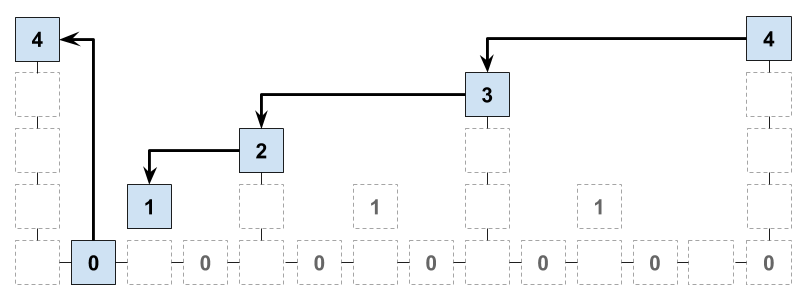
\includegraphics[width=\columnwidth,keepaspectratio]{figures/infix.png}
    \else
        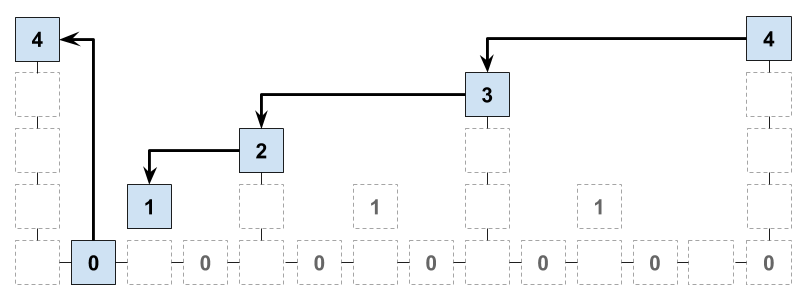
\includegraphics[width=0.7\columnwidth,keepaspectratio]{figures/infix.png}
    \fi
    \label{fig.infix}
\end{figure}

The verification algorithm must then be modified as in
\ref{alg.nipopow-verifier-infix}.

\import{./}{algorithms/alg.verifier-infix.tex}

The algorithm works as before by comparing competing chain prefixes $\pi$ using
the standard $\geq_m$ operator and extracts a best chain prefix $\tilde\pi$ and
$\tilde\chi$. However, it also maintains a blockDAG consisting of blocks from
all proofs. Note that, unlike traditional blockchains, here we have an
\textit{interlink} structure which can potentially be adversarially defined, it
is possible that this collection does not form a blocktree, but a blockDAG with
diamond-shaped topologies. This blockDAG is maintained in the form of a hashmap
in the $\textsf{blockById}$ data structure. Using this, the set of ancestors of
a block present in any of the proofs can be extracted, which is done in the
$\textsf{ancestors}$ method. In the final predicate evaluation, the set of
ancestors of the best blockchain tip is passed to the predicate.

\subsection{Security}
\begin{theorem}
The infix NIPoPoW construction is secure for all infix-sensitive stable
predicates $Q$, except with negligible probability in $\kappa$.
\end{theorem}
\begin{proof}
Assume a typical execution. To prove the security of the construction, it
suffices to show that if all honest verifiers agree on the value of $Q(\chain)$,
then the verifier will output the same value. Assume that all verifiers agree on
the value $v$.

By Theorem~\ref{thm.security} and because the evaluation of $\tilde\pi$ is
identical in the suffix-sensitive and in the infix-sensitive case, we deduce
that $b = \tilde\pi[-1]$ will be an honestly adopted block. Furthermore, due to
the Common Prefix property of backbone, $b$ will belong to all honest parties'
chains and in the same position, as it is buried under $|\tilde\chi| = k$
blocks.

By assumption, at least one honest party $B$ has provided an honest NIPoPoW
$\pi_B$. Let the chain adopted by that honest party during the round in which
the NIPoPoW was produced be $\chain$. Because the predicate $Q$ is infix-sensitive
and stable, this means that $\exists \chain' \subseteq \chain[:-k]:
P_v(\chain')$. Due to $B$ being honest, $\chain' \subseteq \pi_B$. Let
$S = \textsf{ancestors}(b)$ be the ancestors evaluated by the verifier. Clearly
$\chain' \subseteq S$ and therefore $Q(S) = Q(\chain') = v$.
\Qed
\end{proof}

\subsection{Succinctness}
As long as the number of blocks on which the predicate depends is
polylogarithmic with respect to the chain length, our proofs remain succinct.
Specifically, the proof size for the suffix has exactly the same size. Then
the part of the proof that is of interest is the output of the followDown
algorithm. However, notice that this algorithm will on average produce as many
blocks as the difference of levels between $B'$ and $E$, which is at most
logarithmic in the chain size. Hence the proof sizes will be in expectation
$(m + |\chain'|)\log(|\chain|)$, which remains succinct if $|\chain'| \in
O(polylog(|\chain|))$.
